\section{Pilotforsøg - resultater}\vspace{-.75cm}
\textit{Kommentarer og resultater noteret under pilotforsøget}

\subsection{Materiale}
\begin{itemize}
	\item Løbebånd med justerbar hastighed, sikkerhedsbæresele og nødstop.
	\item Motionscykel.
	\item Shimmer3 sensor.
	\item Computer med programmerne:
	\begin{itemize}
		\item Labview.
		\item Shimmer sensing.
		\item NIVISA driver.
	\end{itemize}
\end{itemize}


\subsection{Formål}

\begin{itemize}
	\item Finde ud af hvor stor påvirkning placering af Shimmer3 har på signalet (g-påvirkning/g-krafter?)
	\item Finde ud af om vi tydeligt kan se forskel på aktiviteterne ved hhv. accelerometeret og gyroskopet
	\item Undersøge frekvensindholdet af signalerne
	\item 
\end{itemize}




\subsection{Fremgangsmåde}

\begin{itemize}
	\item Shimmer3 tilsluttes via bluetooth til computeren og kalibreres.
	\item Forsøgspersonen tager bæresele på og den tilpasses.
	\item Shimmer3 sættes i rem og monteres på placering a (højre ankel).
	\item Baseline: Forsøgspersonen står stille på løbebånd i 10 sekunder (dette gemmes mappe: frederik/placeringa_baseline_gang) 
	\item Gang: Løbebåndet tændes og forsøgspersonen begynder at gå, det skrues op på 4,8 km/t, og der ventes til at forsøgspersonen har en homogen cyklus før dataopsamlingen starter (45 sekunder).
	\item Baseline: Forsøgspersonen står stille på løbebånd i 10 sekunder (dette gemmes mappe: frederik/placeringa_baseline_løb)
	\item Løb: (inden dette påbegyndes spørges forsøgspersonen hvordan han/hun har det i forhold til Borg skalaen (forsøget påbegyndes ikke før forsøgspersonen er under 11)) - Løbebåndet tændes og forsøgspersonen begynder at gå, det skrues op på 11,3 km/t, og der ventes til at forsøgspersonen har en homogen cyklus før dataopsamlingen starter (45 sekunder).
	\item Forsøgspersonen står stille på løbebånd i 10 sekunder (dette gemmes mappe: frederik/aktivitet1_/placeringa_baseline_intensitet)
	\item Intensitet: (inden dette påbegyndes spørges forsøgspersonen hvordan han/hun har det i forhold til Borg skalaen (forsøget påbegyndes ikke før forsøgspersonen er under 11)) - Løbebåndet tændes og forsøgspersonen begynder at gå, det skrues op gradvist med 2 km/t pr. 20 sekund, og der ventes til at forsøgspersonen har en homogen cyklus før dataopsamlingen starter (45 sekunder).
	\subitem Det noteres hertil også hvornår forsøgspersonen skifter mellem gang og løb.
	\item Forsøgspersonen sidder stille på kondicyklen i 10 sekunder med højre fod helt i bund (dette gemmes mappe: frederik/aktivitet1_/placeringa_baseline_cykling)
	\item Cykling: (inden dette påbegyndes spørges forsøgspersonen hvordan han/hun har det i forhold til Borg skalaen (forsøget påbegyndes ikke før forsøgspersonen er under 11)) - forsøgspersonen begynder at cykle stille og roligt, og stiger gradvist i hastighed - dette er blot en test på om vi kan se noget, da der ikke var strøm til cyklen.
	
	Dette gentages for alle tre placeringer
\end{itemize}

Intervaller: 
0-20 s: (0-)2 km/t
20-40 s: (2-)4 km/t
40-60 s: (4-)6 km/t
60-80 s:  (6-)8 km/t 
80-100 s: (8-)10 km/t
100-120 s: (10-)12 km/t
120-140 s: (12-)14 km/t
140-160 s: (14-)16 km/t
160-180 s: (16-)18 km/t


\subsection{Noter} 
Frederik placering a: 
\begin{itemize}
	\item Borg skala før gang = 6.
	\item Borg skala før løb = 6.
	\item Borgskala før intensitet = 6.
	\item Skrift fra gang til løb = skift mellem 8 og 10 km/t.
	\item Borg skala før cykling = 6.
\end{itemize}

Frederik placering c: 
\begin{itemize}
	\item Borg skala før gang = 6.
	\item Borg skala før løb = 6.
	\item Borg skala før intensitet = 6.
	\item Skrift fra gang til løb = skift mellem 8 og 10 km/t.
	\item Borg skala før cykling = 8.
	\item Mindre gene ved placering c end placering a dette var gældende for alle aktiviteter. 
\end{itemize}


LS placering a: 
\begin{itemize}
	\item Borg skala før gang = 6.
	\item Borg skala før løb = 6.
	\item Borg skala før intensitet = .
	\item Skrift fra gang til løb = skift mellem  og  km/t.
	\item Borg skala før cykling = .
	\item  
\end{itemize}

Hol øje med hvad package recieve \% er - denne skal gerne være tæt på 100\%.







Vi skal, i det endelige system, være opmærksomme på at det er børn som selv skal sætte den på, så hvor stor er sensibiliteten af sensorerne - påvirker det resultatet hvor højt det sættes og om det hælder/vipper lidt. 

Har vi brug for alle tre akser i accelerometeret/gyroskopet. 
Vi skal gøre det klart at dette også er et forsøg med formålet at finde ud af om vi kan bruge acce elle gyro alene eller om vi vil lave en kobling.

Det står lige pt lidt rodet. 

Skriv grunde til ALT vi gør - hvorfor gør vi det som vi gør og ikke noget andet? 






\begin{figure}[H]
	\centering
	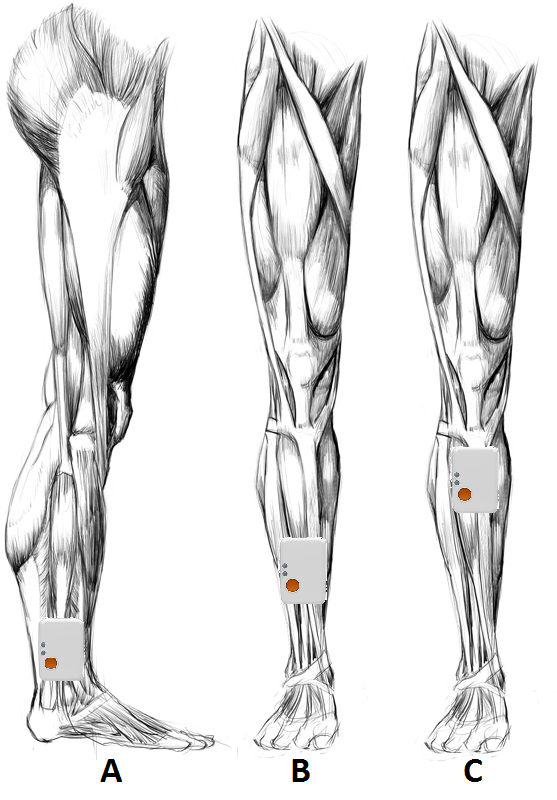
\includegraphics[scale=0.6]{figures/qBilag/Sensor_placering.png}
	\caption{På figuren ses, hvor sensoren skal placeres under pilotforsøget. Placering A viser sensoren siddende proximalt over den laterale malleolus. Placering B illustrerer sensoren, når den er medialt på den ventrale side af tibia. I placering C er sensoren distalt for patella. (Modificeret fra \cite{Perna2016,Shimmer2016})}
	\label{fig:sensor_placering}
\end{figure}
\begin{itemize}
	\item Software punkt...
	\item Kalibrerings punkt....
	\item Forsøgspersonen får fastgjort sensoren i placering A, B eller C - se \figref{fig:sensor_placering}, og gør klar til den pågældende aktivitet ved et stå på kanten af løbebåndet eller sætte sig op på cyklen. Ved aktiviteter på løbebånd skal forsøgspersonen bære sikkerhedsbæresele, som beskytter i tilfælde af fald.
	\begin{itemize}
		\item Ved gang står forsøgspersonen stille på løbebåndet. Optagning af data påbegyndes i 10 sekunder for at optage en baseline for sensorens påvirkning. Herefter træder forsøgspersonen op på løbebåndet og får 20 sekunder til at opnå homogen cyklus i den fysiske udførsel og til, at løbebåndet når op på 4.8 $\sfrac{km}{t}$. Efter disse 20 sekunder optages der yderligere et minut, hvorefter dataoptagelsen stoppes.
		\item Ved løb står forsøgspersonen stille på løbebåndet. Optagning af data påbegyndes i 10 sekunder for at optage en baseline for sensorens påvirkning. Herefter træder forsøgspersonen op på løbebåndet og får 20 sekunder til at opnå homogen cyklus i den fysiske udførsel og til, at løbebåndet når op på 11.3 $\sfrac{km}{t}$. Efter disse 20 sekunder optages der yderligere et minut, hvorefter dataoptagelsen stoppes.
		\item Ved stigning af intensitet skal forsøgspersonen stå stille på løbebåndet mens optagningen påbegyndes og optager en 10 sekunders baseline. Herefter skal løbebåndets hastighed stige fast med et konstant tidsinterval indtil maksspurt er opnået. Dette er en subjektiv vurdering, hvorfor den konstante stigning i hastighed er essentiel og skal noteres i forhold til tid.
		\item Ved cykling skal forsøgspersonen sidde på cyklen og have højre pedal placeret tilnærmelsesvist helt i bund. Der optages en 10 sekunders baseline, hvorefter forsøgspersonen hurtigst muligt og uden at skifte gear skal komme op på 20.9 $\sfrac{km}{t}$. Når dette er opnået, optages signalet i yderligere et minut, hvorefter dataoptagelsen stoppes.
	\end{itemize}
	\item Efter hver måling skal forsøgspersonen restituere i 10 minutter for at sikre, at der ikke sker en kompensering i gang- eller løbecyklus på grund af træthed. %Der tages dog ikke højde for muskeltræthed, da det vurderes, at fysisk aktivitet af denne form ikke vil lede til muskeltræthed inden for disse korte intervaller.\fxnote{Skal vi have en kilde på det her?}
	\item Den pågældende fysiske aktivitet gentages tre gange for hver forsøgsperson, da sensoren skal placeres anderledes for hver gang. Sensoren Shimmer3 skal kalibreres for hvert placeringsskifte og placeringen af sensoren skal markeres på forsøgspersonen. Derved sikres der, at forsøget kan gentages med sammme placering af sensor.
\end{itemize}




Kommentar om hvornår forsøgspersonerne begynder og løbe, så vi kan sammenholde det med graf fra databehandling.